
%%%%%%%%%%%%%%%%%%%%%%%%%%%%%%%%%%%%%%%%%%%%%%%%%%%%%%%%%%%%%%%%%%%%%%%%
%Para las ecuaciones siempre es Ec.(n).
%Para las figuras siempre es Fig.n, incluso en el caption de la figura. Tambien las Tablas
%Para las referencias es [n]
%%%%%%%%%%%%%%%%%%%%%%%%%%%%%%%%%%%%%%%%%%%%%%%%%%%%%%%%%%%%%%%%%%%%%%%%

\documentclass[
reprint,
%notitlepage,
%superscriptaddress,
%groupedaddress,
%unsortedaddress,
%runinaddress,
%frontmatterverbose, 
%preprint,
%showpacs,preprintnumbers,
%nofootinbib,
%nobibnotes,
%bibnotes,
%11 pt,
amsmath,
amssymb,
aps,
pra,
%prb,
%rmp,
%tightenlines %esto hizo el milagro de sacar los espacios en blancos estocásticos (?)
 %prstab,
%prstper,
%floatfix,\textbf{}
]{revtex4-1} %Instalar primero para usarlo. Paquete malo.

%\documentclass[onecolumn, aps, amsmath,amssymb ]{article}
\usepackage{lipsum}  
\usepackage{graphicx}% Include figure files
\usepackage{subfig}
\usepackage{braket}
\usepackage{comment} %comment large chunks of text
\usepackage{dcolumn}% Align table columns on decimal point
\usepackage{bm}% bold math
%\usepackage{hyperref}% add hypertext capabilities
\usepackage[mathlines]{lineno}% Enable numbering of text and display math
%\linenumbers\relax % Commence numbering lines
\usepackage{mathtools} %% Para el supraíndice

\usepackage[nice]{nicefrac}

%%%%%%%El Señor Español%%%%%%%%%%%%%%%%%%%%%%%%%%%
\usepackage[utf8]{inputenc} %acento
\usepackage[
spanish, %El lenguaje.
es-tabla, %La tabla y no cuadro.
activeacute, %El acento.
es-nodecimaldot %Punto y no coma con separador de números
]{babel}
\usepackage{microtype} %para hacerlo más bonito :33 como vos (?) 
%%%%%%%%%%%%%%%%%%%%%%%%%%%%%%%%%%%%%%%%%%%%%%%%%%%
%%%%%%%%% Para que las imágenes se queden dónde las quiero (?
\usepackage{float}
%%%%%%%%%%

%%%%%%%%Cambia a Fig de Figure%%%%%%%%%%
\makeatletter
\renewcommand{\fnum@figure}{Fig. \thefigure} 
\makeatother
%%%%%%%%%%%%%%%%%%%%%%%%%%%%%%%%%%%%%%%%
\raggedbottom

\usepackage{hyperref}
\begin{document}
%%%%%%%%%%%%%%%%%%%%%%%%%%%%%%%%%%Título%%%%%%%%%%%%%%%%%%%%%%%%%%%%%%%%%%%%%%
%%%%%%%%%%%%%%%%%%%%%%%%%%%%%%%%%%%%%%%%%%%%%%%%%%%%%%%%%%%%%%%%%%%%%%%%%%%%%%

\title{Práctica 2: Dinámica de sistemas acoplados }
\author{Evelyn~G.~Coronel}

\affiliation{
Redes~Neuronales - Instituto~Balseiro\\}

\date[]{\lowercase{\today}} %%lw para lw, [] sin date

\begin{abstract}
Soluciones a los ejercicios de la práctica 2 de la materia de Redes Neuronales. En esta práctica se describe  la interacción entre neuronas como sistemas dinámicos acoplados.
\end{abstract} 
\maketitle
%%%%%%%%%%%%%%%%%%%%%%%%%%%%%%%%%%%%%%%%%%%%%%%%%%%%%%%%%%%%%%%%%%%%%%%%%%%%%%%%%%%

\section*{Ejercicio 1}

Las dos poblaciones de neuronas están descritas por las siguientes ecuaciones:
\begin{align}
    \tau \nicefrac{df_e}{dt} &= -f_e + g_{ee} f_e\Theta(f_e) - g_{ei}f_i\Theta(f_i) + I_e\\
    \tau \nicefrac{df_i}{dt} &= -f_i + g_{ie} f_e\Theta(f_e) - g_{ii}f_i\Theta(f_i) + I_i
\end{align}
donde $f_i$ y $f_e$ son las tasas de disparo, $g_{ee}$ y $g_{ii}$ son las conductancias asociadas a la auto-interacción de la neuronas y los términos $g_{ie}$ y $g_{ei}$ son las conductancias de la interacción entre las neuronas.

Sabemos que la solución es estable cuando las derivadas se anulan
\begin{align}
    0= -f_e + g_{ee} f_e\Theta(f_e) - g_{ei}f_i\Theta(f_i) + I_e\\
    0= -f_i + g_{ie} f_e\Theta(f_e) - g_{ii}f_i\Theta(f_i) + I_i
\end{align}

Considerando que las tasas de disparo $f_e$ y $f_i$ son positivas, donde $0$ implicaría la ausencia de spikes, y las conductancias  son mayores o iguales a 0,  las condiciones de estabilidad quedan como
\begin{align}
     (1 -g_{ee}) f_e &= -g_{ei}f_i + I_e \label{fe}\\
    (1 + g_{ii}) f_i &=  g_{ie} f_e  + I_i
\end{align}

Por lo que finalmente llegamos a un sistema de ecuaciones lineales para las tasas. Resolviendo este sistema, las tasas son iguales a 
%En cambio para la tasa $f_e$ dependiendo del valor de la conductancias puede tomar un valor negativo; por hipótesis asumimos que $f_e \ge 0$, esto implica que la actividad o la cantidad de spikes es nula.
\begin{align}
     f_i = \frac{g_{ie}I_e + I_iA}{g_{ei}g_{ie}+ AB}\\
     f_i = \frac{g_{ei}I_i + I_eB}{g_{ei}g_{ie}+ AB} 
\end{align}
donde $A= 1 - g_{ee}$ y $B=1+g_{ii}$. Como buscamos que las tasas sean positivas, implica que 

\begin{align}
     \frac{g_{ie}I_e + I_i -g_{ee}I_i }{1+g_{ei}g_{ie} - g_{ii}g_{ee} -g_{ee}-g_{ii}} > 0\\
     \frac{g_{ei}I_i + I_e +g_{ii}I_e }{1+g_{ei}g_{ie} - g_{ii}g_{ee} -g_{ee}-g_{ii}} > 0 
\end{align}


\section*{Ejercicio 2}

\subsection{Introducción}

Las neuronas del tipo Hogdkin-Huxley se basan las ecuaciones presentadas en \cite{HH}. En este trabajo, se agrega un parámetro más, $s$, que corresponde a la función inhibitoria \cite{syn}, usado para modelar la inhibición sináptica. Este parámetro es descrito mediante la siguiente ecuación diferencial,
\begin{align}
    \frac{ds}{dt}&= \frac{s_\infty(V) - s}{\tau}\\
    s_\infty(V)&= 0.5(1+tanh(\nicefrac{V}{5})),
\end{align}
donde $V$ es el potencial de  la neurona y $\tau$ es el tiempo característico asociado a la inhibición. En este trabajo se considera  $\tau = 3\,$ms.

Para estudiar la interacción entre dos neuronas de Hogdkin-Huxley, consideramos que están conectadas simétricamente, es decir, la corriente $I(t)$ para ambas tiene la siguiente forma
\begin{align}
    I(t)            &= I_0 + I_{syn}(t)\\
    I_{syn}(t)      &= -g_{syn}s(t)(V-V_{syn}),
\end{align}
donde la corriente $I_0$ debe ser un valor tal que para las dos neuronas produzcan spikes periódicamente, $s(t)$ es el parámetro descrito anteriormente, $g_{syn}$ es la conductancia asociada con la entrada sináptica y $V_{syn}$ es el potencial sináptico.

\subsection{Simulaciones}

En esta sección se varía el parámetro $g_{syn}$ entre $0$ y 2 ${\text{mS}}/{\text{cm}^2}$ con $\Delta g_{syn}=0.02\,{\text{mS}}/{\text{cm}^2}$ para 100 iteraciones. En cada interación se mantiene fijo un valor para $V_{syn}$. La simulación utiliza un variación de tiempo de $\Delta t =  0.005\,$ms y realizan $50000$ interaciones, para un total de 250\,ms. Además para cada valor el $g_{syn}$, las condiciones iniciales de las neuronas son tales que las mismas no estén en fase. Estás condiciones están dadas en la Tabla~\ref{tab:ini}. 
    \begin{table}[H]
    \centering
    \begin{tabular}{c| c| c}
    {\bf Variable }& {\bf Neurona 1} & { \bf Neurona 2} \\ \hline
        V [mV]     & 80.0            & -80.0               \\  \hline
        m          & 0.1             & 0.1              \\  \hline
        h          & 0.3             & 0.7               \\  \hline
        n          & 0.1             & 0.3               \\  \hline
        s          & 0.0             & 0.0               \\      
    \end{tabular}
    \caption{Condiciones iniciales las neuronas del tipo Hodgkin-Huxley.}   
         \label{tab:ini}
    \end{table}
Los parámetros adimensionales m, h y n están asociados a los canales de activación e  inactivación de sodio y al canal de potasio respectivamente.

   \subsubsection{Caso \texorpdfstring{$V_{syn}= 0\,\text{mV}$}{}   con  \texorpdfstring{$I_0 = 15\,\mu A$}{}}

    En la Fig.\,\ref{fig:des_fre} se observa las curvas del voltaje y del desfase de las dos neuronas involucradas en función de la conductancia $g_{syn}$. Se observa la disminución de la frecuencia de las neuronas con el aumento del valor de $g_{syn}$, debido a que la corriente $I_{syn}$ disminuye en media la corriente dentro de la neurona, esto es consistente con la curva f-I de las neuronas del tipo HH, donde la frecuencia aumenta con la corriente en la neurona.  

        \begin{figure}[H]
            \centering
            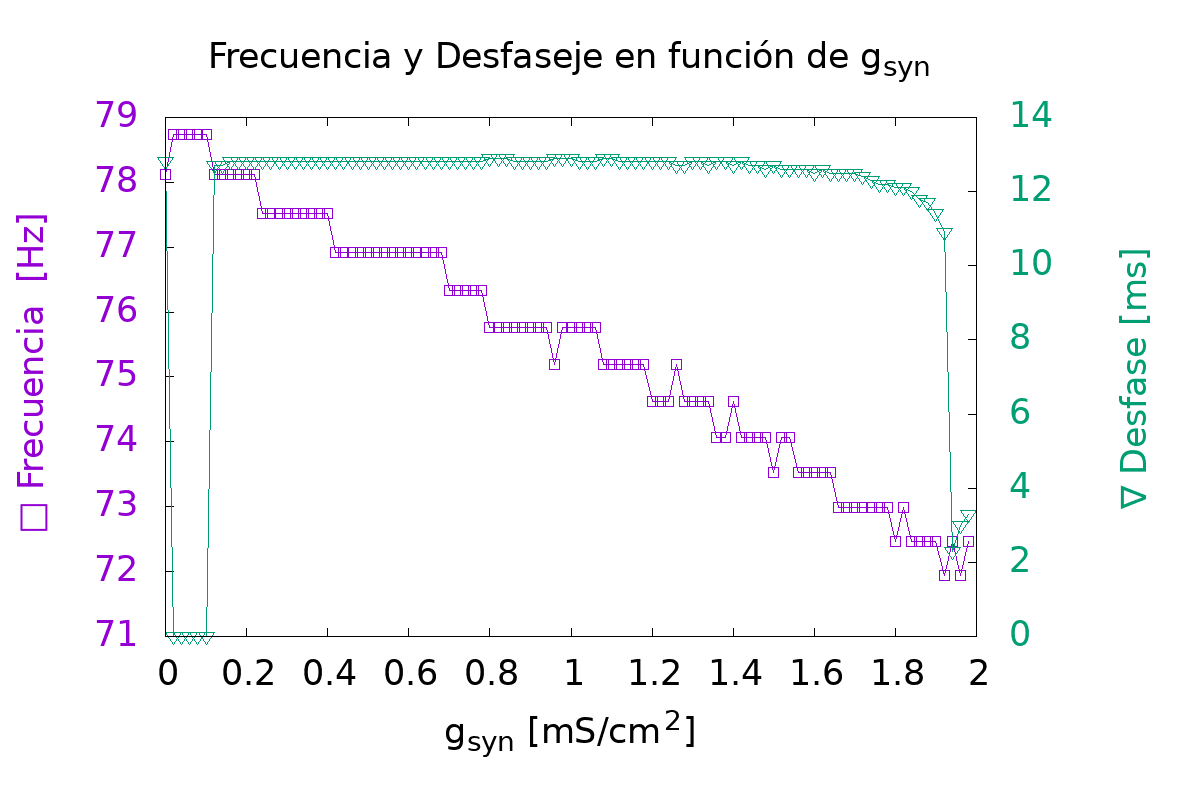
\includegraphics[width=0.5\textwidth]{../Graficos/current_15.png}
            \caption{Desfase y frecuencia de las neuronas en función de $g_{syn}$. Los valores de la frecuencia están a la izquierda del gráfico mientras que los valores del desfase se muestran a la derecha.}
            \label{fig:des_fre}
        \end{figure}  

    Analizando la curva del desfase, se observa que este valor disminuye a media que aumenta el valor de $g_{syn}$. Por lo que aumentando este parámetro, puedo lograr que las dos neuronas se sincronicen.

       El valor de la corriente, así como los spikes en función del valor de $g_{syn}$ pueden verse en \footnote{\url{https://github.com/astrocronopio/NN_IB/blob/master/pr-rn-2/Graficos/current_15.gif}}

  



    \subsubsection{Caso \texorpdfstring{$V_{syn}= -80\,\text{mV}$}{}   con  \texorpdfstring{$I_0 = 15\,\mu A$}{}}

    En la Fig.\,\ref{fig:des_fre_in} se observa una tendencia creciente en el valor de la corr


    \begin{figure}[H]
            \centering
            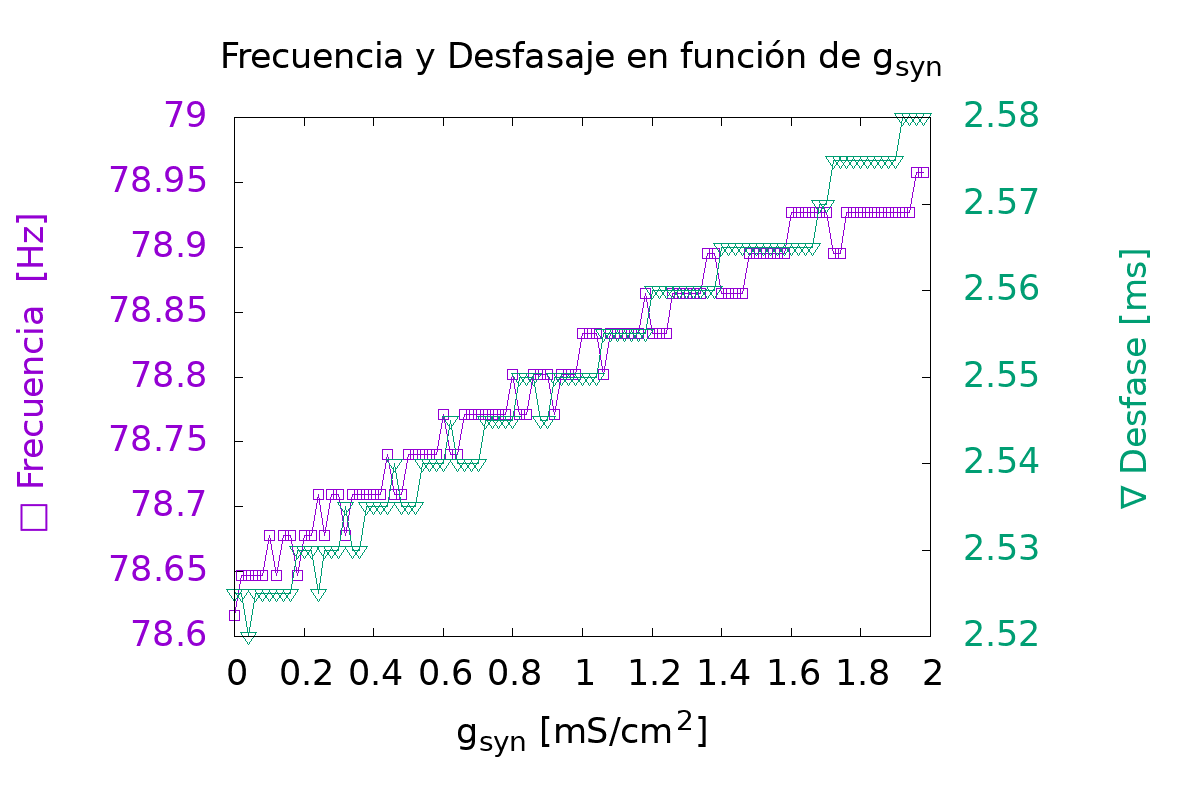
\includegraphics[width=0.5\textwidth]{../Graficos/current_15_in.png}
            \caption{Desfase y frecuencia de las neuronas en función de $g_{syn}$ para $V_{syn}=-80\,$mV.}
            \label{fig:des_fre_in}
        \end{figure}



\begin{thebibliography}{50}
%\onecolumn
\bibitem{HH} Izhikevich E. M. Capítulo 2. Sección 2.3: Hodgkin-Huxley Model en {\sl Dynamical Systems in Neuroscience: The Geometry of Excitability and Bursting} (2005).  The Neurosciences Institute.
\bibitem{syn} Börgers C, Krupa M, Gielen S. The response of a classical Hodgkin-Huxley neuron to an inhibitory input pulse. J Comput Neurosci. 2010;28(3):509–526. doi:10.1007/s10827-010-0233-8
\end{thebibliography}

\end{document}